\chapter{Setup of the physical Environment}
The production line at \ac{SPC} is planned to produce steering knuckles with \ac{FRC}.

\section{Steps in the Production Line}
The planned production line consists of several steps that can be seen in figure \ref{fig:ProdLineSchem}. A visual representation from the simulation with Visual Components can be found in figure \ref{fig:ProdLineVisComp}.

\begin{figure}[H]
	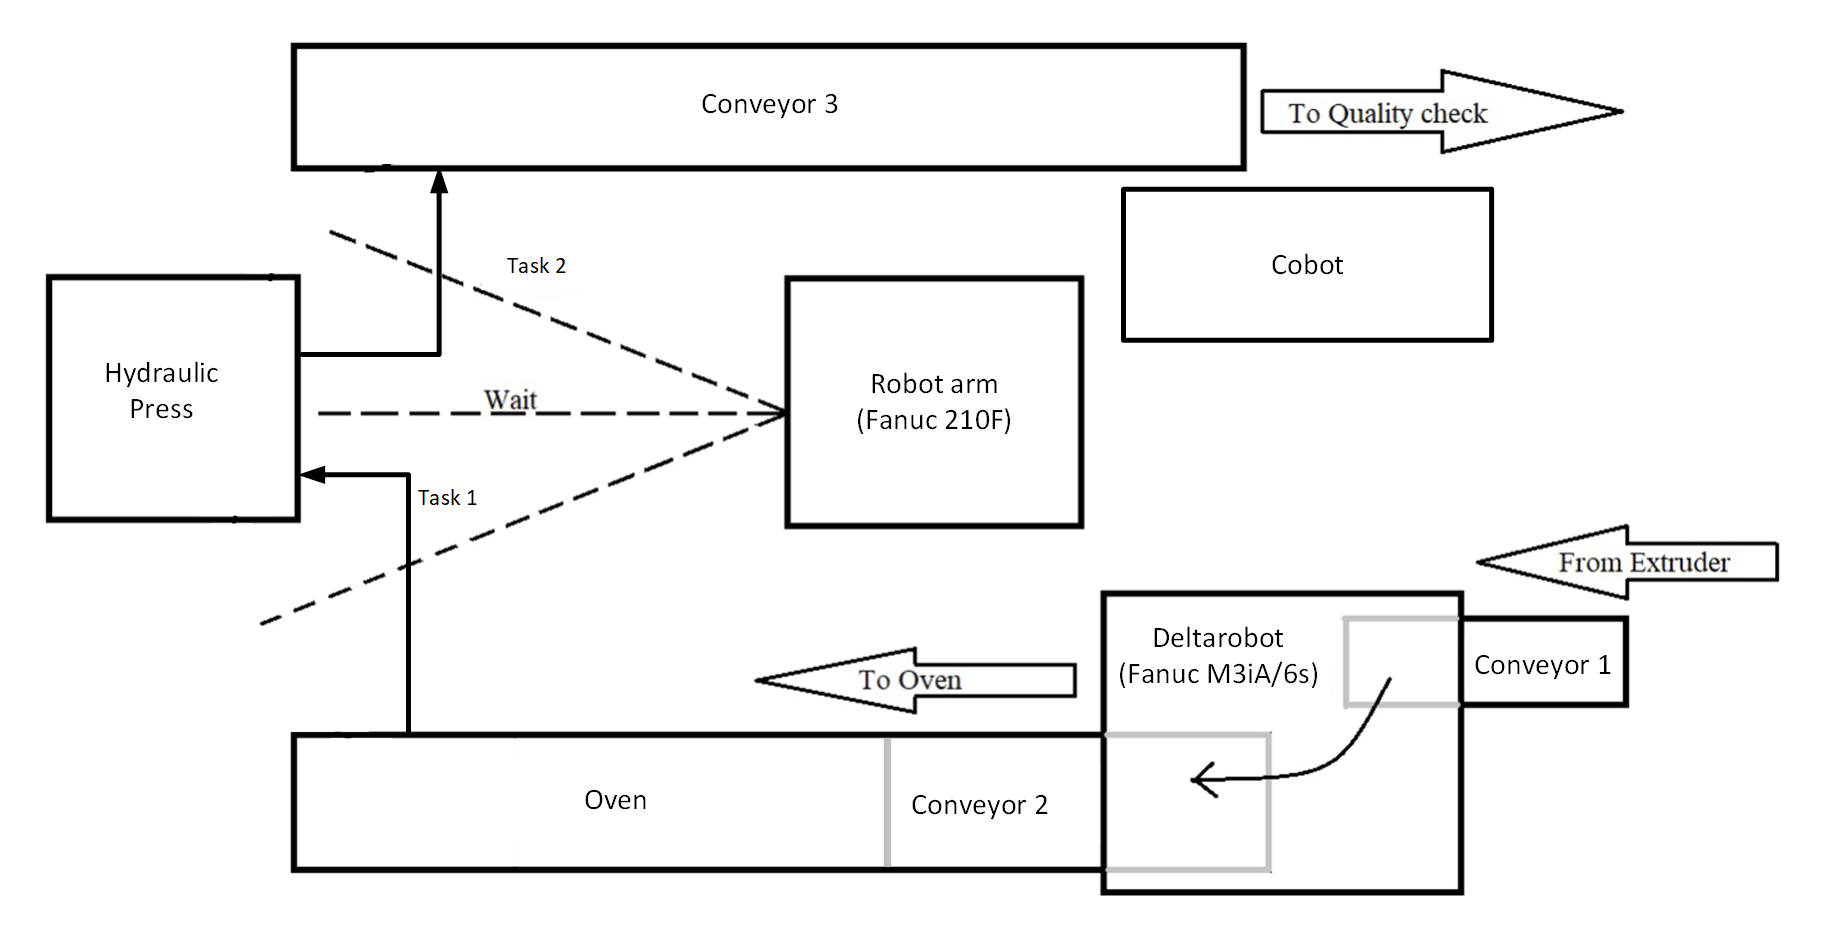
\includegraphics[
	width=\linewidth,
	center,
	keepaspectratio,
	]{ProductionLineSetup/drawing}
	\caption{Schematic of the floorplan \cite{AliyaThesis}}
	\label{fig:ProdLineSchem}
\end{figure}

\begin{figure}[h]
	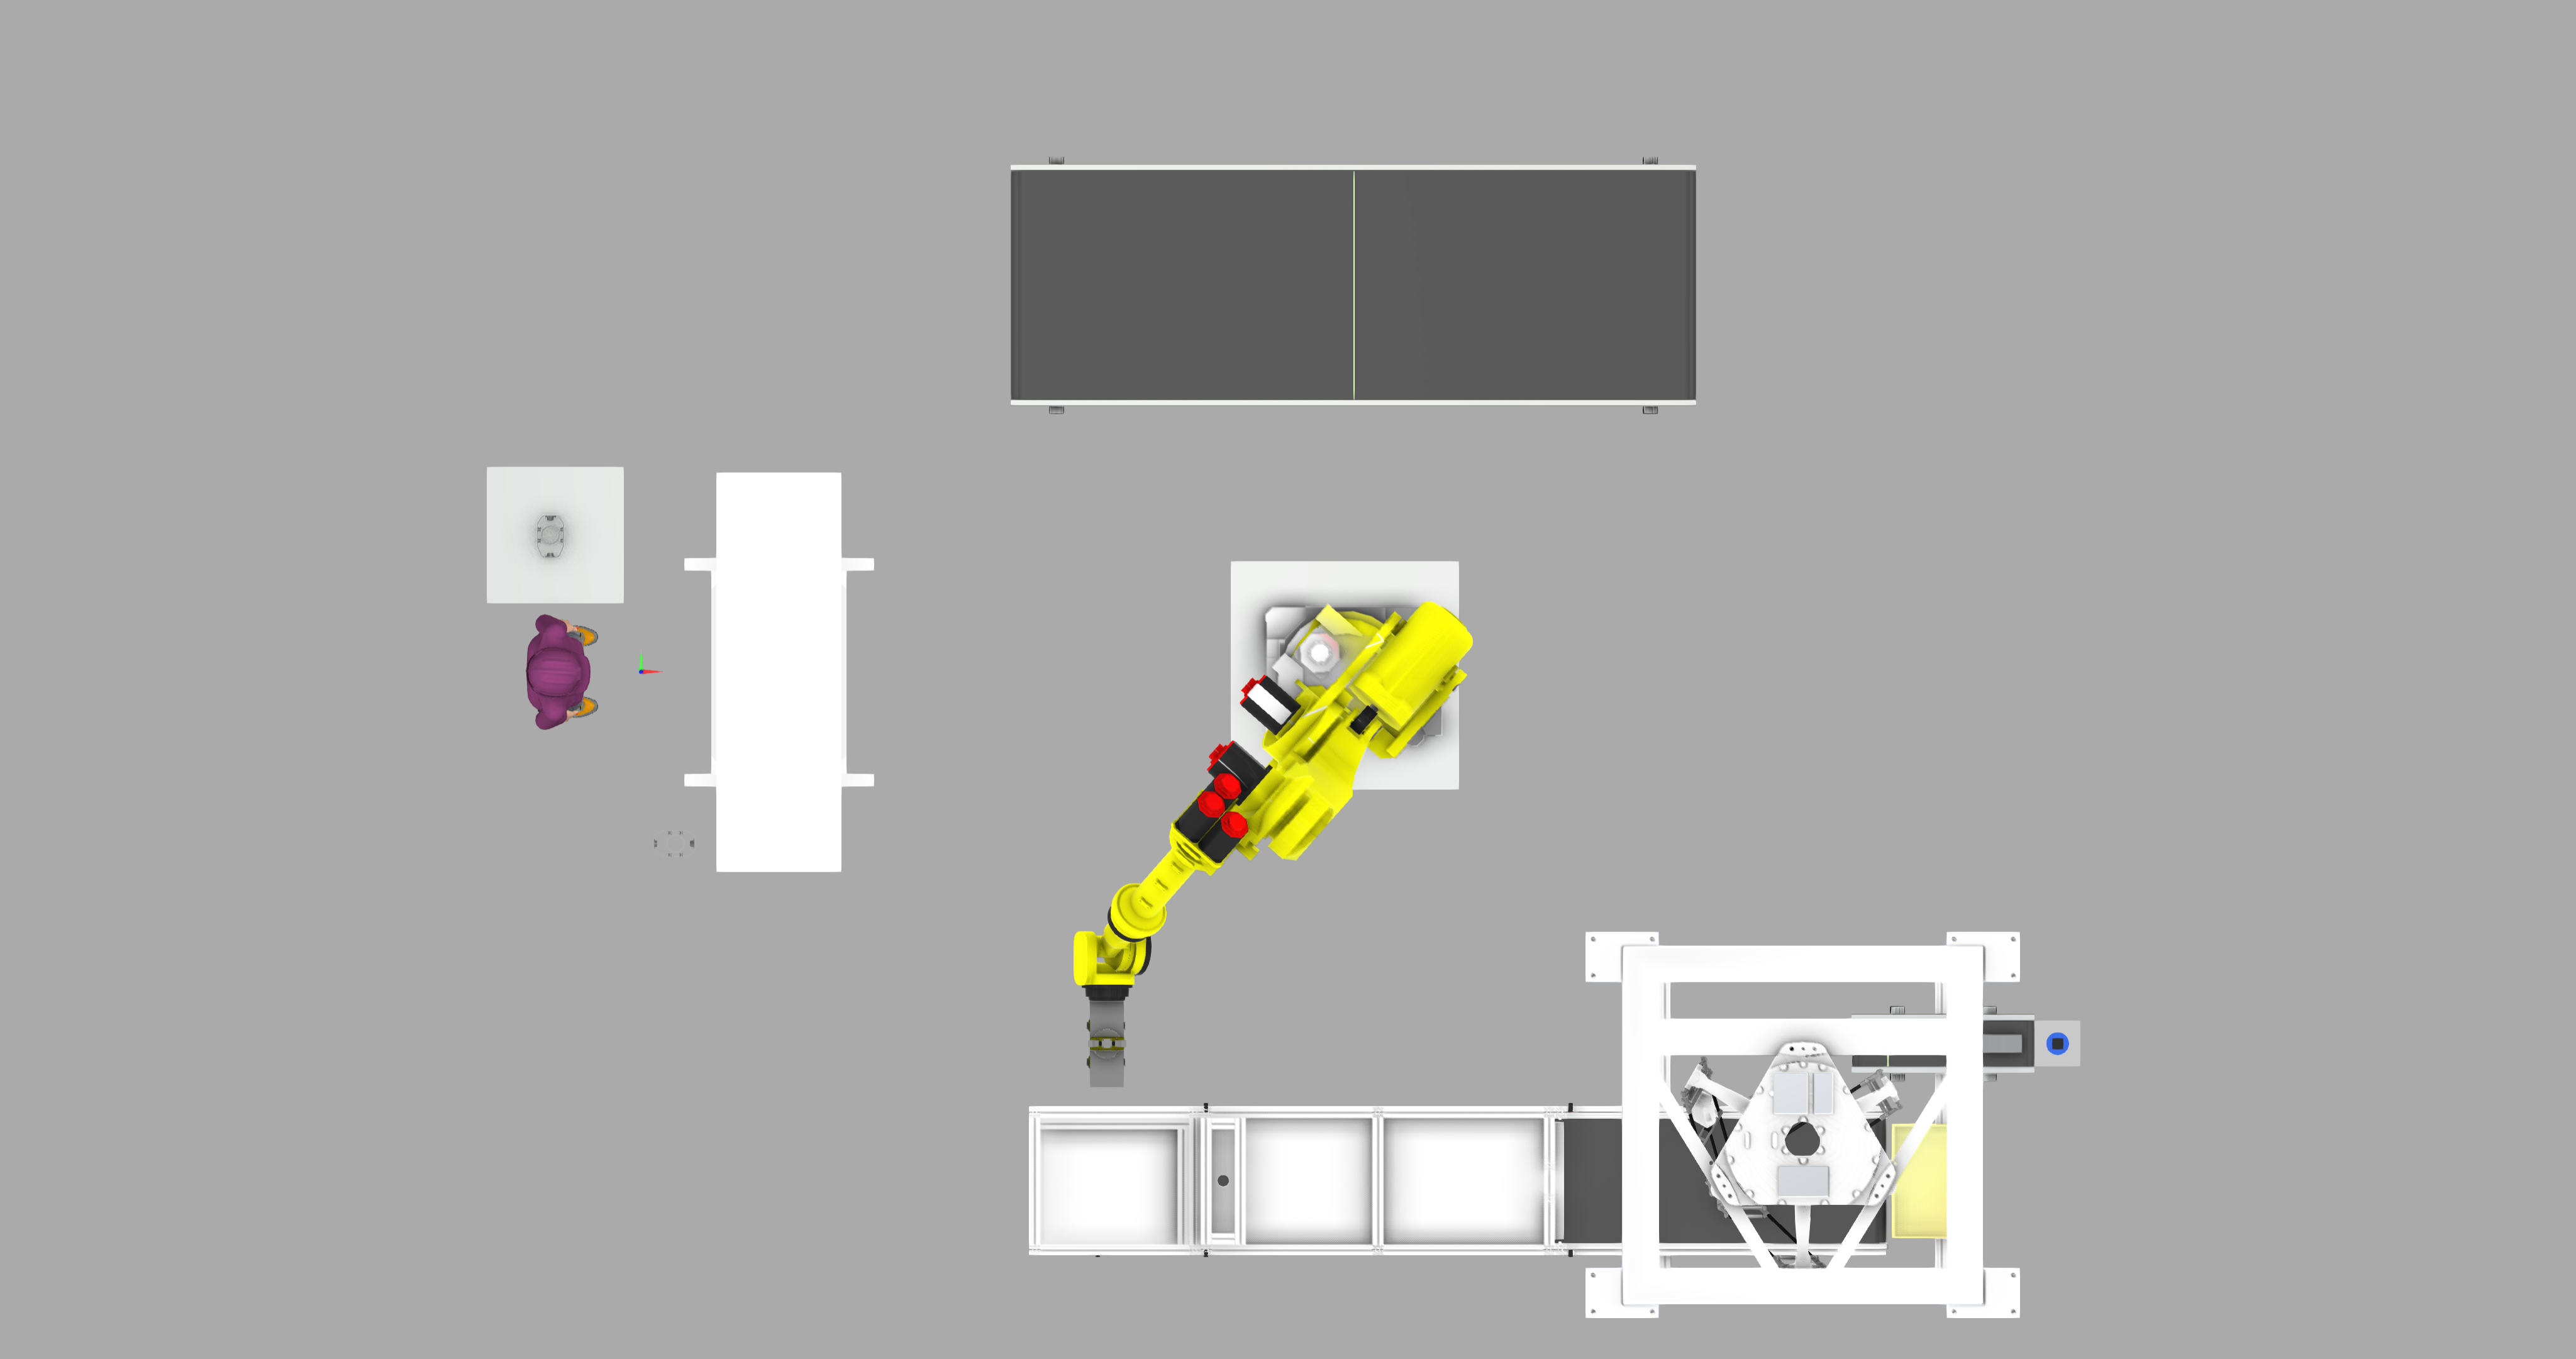
\includegraphics[
	width=\linewidth,
	center,
	keepaspectratio,
	]{ProductionLineSetup/Rendering}
	\caption{Top view of Production line layout, rendered with Visual Components \cite{AliyaThesis}}
	\label{fig:ProdLineVisComp}
\end{figure}



\paragraph{Extruder} \label{sec:extruder}
\ac{FRP} raw material pellets are fed into an extruder. 
Alternatively, reprocessed material from steps down the production line is fed into the extruder.
The extruder melts the raw material and releases it at its hot end. 
At the hot end of the extruder, the material is portioned into blops of 300g each by a guillotine.

\paragraph{Conveyor 1} \label{sec:conveyor1}
The first conveyor belt transports the \ac{FRP} material blops from the output of the \nameref{sec:extruder} to the \nameref{sec:Deltarobot}. At the end of the coveyor belt is a proximity sensor to detect incoming material.

\paragraph{Deltarobot} \label{sec:Deltarobot}
After a signal is given from the proximity sensor of \nameref{sec:conveyor1}, a  Fanuc M-3iA/6S 4-axis Delta-robot picks up the material and weighs it with a load cell built into the gripper of the robot. 
If the weight of the material is out of the desired range, it is discharged into a waste bin and recycled with the \nameref{sec:extruder}.
If the weight of the material is within an acceptable range, it is placed on \nameref{sec:conveyor2}.
When placing the material on conveyor 2, the placement position and other data are communicated to processes further down the line.
If needed, multiple blops of material can be stacked to the desired height while \nameref{sec:conveyor2} keeps moving.


\paragraph{Conveyor 2} \label{sec:conveyor2}
The second conveyor belt transports the sorted and arranged \ac{FRP} material from the \nameref{sec:Deltarobot} through the \nameref{sec:oven}. 

\paragraph{Oven}\label{sec:oven}
The oven takes in the blops of \ac{FRP} material, and brings them up to the desired temperature with induction heaters. The material is then stored in a buffer zone separated with doors from the oven and the heating chamber where the material is kept at temperature. When the \nameref{sec:HydraulicPress} is ready, a door in the buffer zone opens for the Robot arm to pick up the material.

%The oven can be separated into several zones:
%\subparagraph{Oven entrance}
%With the position data provided by the \nameref{sec:Deltarobot} and the \nameref{sec:conveyor2} speed, the oven door at the entrance can open at the right time to take in the material.
%\subparagraph{Heating chamber} \label{sec:HeatingChamber}
%In the heating chamber, the material is brought to the desired temperature with several induction heaters.
%\subparagraph{Internal door}
%With the position data provided by the \nameref{sec:Deltarobot} and the \nameref{sec:conveyor2} speed, a door inside the oven can open at the right time to take in the material.
%\subparagraph{Buffer zone} \label{sec:BufferZone}
%A buffer zone, separated from the \nameref{sec:HeatingChamber} provides an area to keep the material at the desired temperature until it can be processed further.
%\subparagraph{Oven output}
%When the \nameref{sec:HydraulicPress} is ready, a door in the \nameref{sec:BufferZone} opens for the Robot arm to pick up the material.

\paragraph{Robot arm} \label{sec:RobotArm}
The robot arm has two tasks:
\begin{enumerate}
	\item After a signal is given from the \nameref{sec:HydraulicPress}, the Fanuc 210F 6axis robot arm picks up the hot \ac{FRP} material stack from the buffer zone and places it in a \nameref{sec:HydraulicPress} with a specialized gripper. 
	After placing the part, the robot changes its gripper tool, and waits for its second task.
	\item When the forming process in the \nameref{sec:HydraulicPress} is finished, the mould opens, and the robot arm %and the same robot arm as in \nameref{sec:RobotArm1}
	can use another gripper to pick up  the \ac{FRP}-part and place it on \nameref{sec:conveyor3}.
	After placing the part, the robot changes its gripper tool, and waits for its first task
\end{enumerate}


%\paragraph{Robot arm task 1} \label{sec:RobotArm1}
%After a signal is given from the \nameref{sec:HydraulicPress}, a Fanuc 210F 6axis robot arm picks up the hot \ac{FRP} material stack from the buffer zone and places it in a \nameref{sec:HydraulicPress} with a specialized gripper.
%After placing the part, the robot changes its gripper tool, and waits for its second task, see \nameref{sec:RobotArm2}.

\paragraph{Hydraulic press} \label{sec:HydraulicPress}
After all material is placed and the \nameref{sec:RobotArm} has completely withdrawn from the press in a safe distance, the press will close the heated mould to give the \ac{FRP} material its desired shape with heat and pressure. After an estimated cycle time of 1 minute, the press opens and the finished part can be picked up.

%\paragraph{Root arm task 2} \label{sec:RobotArm2}
%When the forming process in the \nameref{sec:HydraulicPress} is finished, the mould opens, and the same robot arm as in \nameref{sec:RobotArm1} can use another gripper to pick up  the \ac{FRP}-part and place it on \nameref{sec:conveyor3}.
%After placing the part, the robot changes its gripper tool, and waits for its first task, see \nameref{sec:RobotArm1}.

\paragraph{Conveyor 3}\label{sec:conveyor3}
The third conveyor belt transports the formed part from the press to the \nameref{sec:Cobot}.

\paragraph{Cobot} \label{sec:Cobot}
When the material arrives at the cobot, it is picked up, and presented to a camera system for analysation. If the part fulfils the desired properties, it is given to further processing steps and packing.
In case, it does not fulfils the desired properties, it can be recycled with the \nameref{sec:extruder}.

\section{Notes on choice of robot} %should go to appendix
The robot was chosen for this production line, as it provides a long reach. The arm without any \ac{EOAT} can reach a full circle with a radius of $2655 [\textit{mm}]$ with its mounting plate. Also the overall weight of $1240 [\textit{mm}]$ allows for reasonably fast movements between $90-190 [\textit{°/sec}] $ depending on the axis while still giving a payload capacity of $210 [\textit{Kg}]$ at the mounting plate.\cite{210FDatasheet}
This high payload capacity is not needed directly, but it provides enough room for complex gripper designs, and provides room for future uses of the device.

\section{Status of the production line at beginning of project}
At the start of this thesis work, the \nameref{sec:HydraulicPress} was already fixed to the ground. 
\nameref{sec:Deltarobot},\nameref{sec:conveyor2}, and the robot arm were roughly placed at their final positions.
No gripper tools were available for either robots.
The \nameref{sec:extruder}, \nameref{sec:oven}, \nameref{sec:conveyor1}, \nameref{sec:Cobot} and \nameref{sec:conveyor3} were not available.
Electricity for the machines was not made available.
A safety-fence was not set up.

\section{Status of the production line at the end of thesiswork}
At the end of the project, the robots are positioned at a preferable position for their intended use. Interaction between press and robot arm were tested. Grippers were being developed in \ac{CAD}, and some standardized pneumatic grippers were tested on the robot arm for pick and place operations. \nameref{sec:conveyor2} was positioned, and fixed to the ground. Also, it was also tested with a Profinet-controlled variable frequency drive via \ac{PLC}. A heat resistant belt still needs to be mounted. An \nameref{sec:extruder} was delivered, but still needs to be commissioned, tested and modified. 
An \nameref{sec:oven}, \nameref{sec:conveyor1}, \nameref{sec:conveyor3} and a \nameCref{sec:Cobot}-station are still missing.
A preliminary safety fence with no electronic safeguard has been set up. 


\section{Set up process of Robot arm}

\subsection{Positioning}
In order to integrate the robot arm into the production line, it needed to be mounted at its final position. This position was determined with a floorplan. To create the floorplan, the three members of SPC responsible for the \nameref{sec:Deltarobot}, the \nameref{sec:conveyor2}/\nameref{sec:oven} and the robot arm worked out the positions of their machines with the help of Qing Groep. At Qing, the production line was modelled in \ac{VC}. With \ac{VC} different positions for these machines could be tested. 
Simple pick and place programs could be simulated in that environment.
These movements could be inspected an varied to allow a smooth and fast transfer of material.
As the \nameref{sec:HydraulicPress} was already fixed to the ground, all other positions were determined relative to the press.
After estimating good positions via \ac{VC} with respect to the movement range of the robot arm, the outlines of the machine feets were measured with a laser distance measurement system and marked on the floor.
After placing the robots with a forklift on the desired positions, the actual positions were measured again with the laser distance measurement system, documented in an excel sheet and tested again in VC. 
As the differences between actual and desired position were minimal, the simulations in VC did not show any problems.
The robot arm and the other machines was then bolted down in the ground. 

\subsection{Comissioning}
After the robot arm was positioned at its desired position, it could be plugged into the accompanying Fanuc R-30iA controller and was provided with electricity. 
This step was delayed a lot, as a safe and powerful enough electrical installation could not be provided by the \ac{MIC} from the beginning of the project.
After the robot and controller were running, the basic functions as found in the manuals could be tested. 
Manuals and configuration files were delivered by the previous owner, IRSA Robotics, on a set of \ac{usb}-sticks. 
These \ac{usb} sticks had all kinds of manuals and configuration files for both robots without any context and order on them. 
An extensive search and ordering was needed to get the right manuals.
Additionally, the previous owner had left a non-functional configuration on the robot, that was overcome by a complete factory reset with the help of Fanuc customer service.
When these issues were overcome, the robots could be calibrated. As described in the manual, the robots have calibration markings. With these markings aligned, a calibration could be made with the \gls{ipendant}.




\subsection{Fieldbus and Network setup}

For the state of this thesis-work, the field bus and network- installation consists of following parts:
\begin{itemize}
	\item \ac{PLC}
	\item \ac{HMI}-Display
	\item \ac{VFC} for conveyor belt
	\item R-2000 iA Mate Controller for Delta robot
	\item R-2000 iA Controller for Robot arm
	\item Several student notebooks for configuration, monitoring and control of the machines
\end{itemize}

Additionally following devices are Planned:
\begin{itemize}
	\item \ac{DDS} (eventually consisting of several distributed nodes)
	\item cameras for process monitoring 
	\item Controller for \nameref{sec:Cobot}
	\item Controller for Extruder and Feeding system
	\item Part inspection system
	\item various sensors
\end{itemize}

The physical layer of the network and field bus is based on Ethernet. A basic connection to the PLC via Profinet as well as to the network via IP/Etherent at \ac{SPC} was achieved.\\
\\
The currently loaded configurations for network and field bus can be found in the \ac{ipendant}.

\subsection{Cooperation with Qing}
Together with the company Qing, an event about digital twinning was hosted at the \ac{SPC}. In the preparation of this event, a program for loading the press with the robot arm and unloading the finished product was developed. This program can be found in the appendix \fullref{TPprogram210F}.